\documentclass[a4paper,11pt]{article}

\usepackage[finnish]{babel}
\usepackage{xcolor}
%\usepackage[framemethod=TikZ]{mdframed}
\usepackage[utf8]{inputenc}
\usepackage[top=1.5cm, bottom=1.5cm]{geometry}
\usepackage{amsfonts,amsmath,amssymb,amsthm,enumitem}
\usepackage{microtype}
\usepackage{pgf}
\usepackage{tikz}
\usepackage{environ}
\usepackage{color}
\usetikzlibrary{arrows,automata}

\setenumerate{listparindent=\parindent}

\newtheorem*{claim}{Väite}
\theoremstyle{definition}
\newtheorem*{lemma}{Lemma}
\newtheorem*{definition}{Määritelmä}

\newtheorem{exercisethm}{Tehtävä}
%\colorlet{shadecolor}{cyan!8}
%\newenvironment{exercise}
%{\begin{mdframed}[roundcorner=10pt]\begin{exer}}
        %{\end{exer}\end{mdframed}}

\newcommand{\set}[1]{{\left\{ #1 \right\}}}
\newcommand{\ceil}[1]{{\left\lceil#1\right\rceil}}
\newcommand{\Nat}{\mathbb{N}}

\newcommand{\fixme}[1]{\textcolor{red}{FIXME: #1}}

\tikzstyle{mybox} = [draw=none, fill=cyan!9, rectangle,
  rounded corners, inner sep=10pt, inner ysep=20pt]

\NewEnviron{exercise}{%
  \vspace{5mm}
  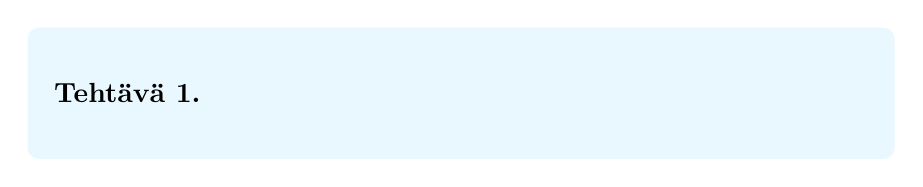
\begin{tikzpicture}
    \node[mybox]
    {\begin{minipage}{0.85\textwidth}
        \begin{exercisethm}
          \BODY
        \end{exercisethm}
    \end{minipage}};
  \end{tikzpicture}
}

\title{Pumppauslemmaopas}
\author{Juhana Laurinharju \and Jani Rahkola}

\begin{document}

\belowdisplayskip=11pt
\abovedisplayskip=11pt
\belowdisplayshortskip=11pt
\abovedisplayshortskip=11pt

%\thispagestyle{empty}
\maketitle

\section*{Pumppauslemma}
%\pagestyle{myheadings}
%\markright{Jee}

Jokaisella säännöllisellä kielellä on seuraava \emph{pumppauslemmana} tunnettu
ominaisuus.

\begin{definition}[pumppauslemma]
    Olkoon $A$ säännöllinen kieli. Tällöin $A$:lla on jokin
    pumppauspituus $p \in \Nat$, $p > 0$. Nyt kaikki vähintään $p$:n
    mittaiset merkkijonot $s \in A$, $|s| \geq p$ voidaan jakaa
    kolmeen osaan $s = xyz$ siten, että seuraavat kolme ehtoa ovat
    voimassa.

    \begin{enumerate}
        \item
          $xy^iz \in A$ jokaisella $i \in \Nat$, erityisesti myös kun
          $i = 0$.
        \item
          $|y| > 0$, eli toistettava osa $y$ ei saa olla tyhjä
          merkkijono $\varepsilon$.
        \item
          $|xy| \leq p$
    \end{enumerate}
\end{definition}

Otetaan tästä konkreettinen esimerkki. Kieli
\begin{equation*}
    A = L(a^*b^*)
\end{equation*}
on säännöllinen ja sillä on täten jokin pumppauspituus $p$. Tä\-män kielen
kohdalla eräs mahdollinen pumppauspituus on ${p = 3}$. Tämän pumppauspituuden
saa esimerkiksi siitä, että kielen voi tunnistaa deterministisellä äärellisellä
automaatilla jossa on kolme tilaa. Tarkastellaan jotain riittävän pitkää kielen
$A$ merkkijonoa. Valitaan ${s = abbb}$. Nyt pumppauslemman nojalla löytyy
\emph{jokin} jako ${s = xyz}$, jolle yllä olevat kolme ehtoa pätevät.

Tarkastellaan merkkijonon $s$ mahdollisia jakoja.

\begin{itemize}
    \item Kokeillaan ensin seuraavaa jakoa:
        \begin{align*}
            x            & = \varepsilon \text{,}  \\
            y            & = ab            \\
            \text{ja } z & = bb
        \end{align*}
        %
        Nyt ehdot 2 ja 3 ovat voimassa, mutta ensimmäinen ehto ei täyty, sillä
        esimerkiksi merkkijono $xyyz = ababbb$ ei kuulu kieleen $A$.

    \item Ensimmäinen jako ei siis täyttänyt kaikkia pumppauslemman ehtoja.
        Pumppauslemma ei kuitenkaan takaa, että nämä ehdot täyttyisivät
        jokaisella jaolla. Ainoa tae on se, että löytyy jokin ehdot täyttävä
        jako. Tällainen on esimerkiksi seuraava jako:
        %
        \begin{align*}
            x              & = a \textrm{,} \\
            y              & = b \\
            \textrm{ja } z & = bb
        \end{align*}
        Nyt $|xy| = 2 \leq p$, $|y| = 1 > 0$. Entä miltä näyttää merkkijono
        $xy^iz$? Tarkastellaan tätä ensin $i$:n arvoilla $0$, $1$ ja $2$:
        %
        \begin{align*}
            xy^0z & = xz  = abb \in A \\
            xy^1z & = xyz = abbb \in A \\
            xy^2z & = xyyz = abbbb \in A
        \end{align*}
        %
        Ja yleisessä tapauksessa, kun $i \in \Nat$, niin
        %
        \begin{equation*}
            xy^iz = ab^ibb = ab^{i+2} \in L(a^*b^*) = A
        \end{equation*}
\end{itemize}

\begin{exercise}
    Olkoon
    %
    \begin{equation*}
        A = L((ab)^*)
    \end{equation*}
    %
    säännöllinen kieli. Tällä kielellä on pumppauspituus $p = 2$. Valitaan
    kielestä merkkijono
    %
    \begin{equation*}
        s = ababab
    \end{equation*}
    %
    joka on pidempi kuin pumppauspituus $p = 2$.  Anna kaikki merkkijonon $s$
    jaot $s = xyz$ jotka täyttävät pumppauslemman ehdot $2$ ja $3$, eli 
    %
    \begin{align*}
        |y|  & > 0 \textrm{ ja} \\
        |xy| & \leq p \text{.}
    \end{align*}
\end{exercise}

\begin{exercise}
    Mitkä edellisen tehtävän jaoista $s = xyz$ toteuttavat pumppauslemman
    ensimmäisen ehdon? Ensimmäinen ehto on
    %
    \begin{equation*}
        xy^iz \in A \text{ kaikilla } i \in \Nat
    \end{equation*}
    %
    eli keskikohtaa $y$ voi toistaa.
\end{exercise}

\section*{Pumppauslemman käyttäminen}

Pumppauslemma on hyödyllinen, koska sillä voidaan näyttää monia kieliä
epäsäännöllisiksi. Mutta kuinka tämä onnistuu työ\-ka\-lul\-la, joka ei puhu
mitään epäsäännöllisistä kielistä? Pumppauslemman jos-niin
rakenteeseen piiloutuu kuitenkin myös väite epäsäännöllisyydestä.
Seuraava lemma on nimittäin yh\-tä\-pi\-tä\-vä pumppauslemman kanssa.

\begin{lemma}
  Olkoon $A$ jokin kieli. Oletetaan lisäksi, että kaikilla
  luonnollisilla luvuilla $p > 0$ jotain kielen $A$ merkkijonoa $s$,
  $|s| \ge p$ ei voida jakaa \emph{millään tapaa} kolmeen osaan $s =
  xyz$ siten, että seuraavat ehdot olisivat voimassa:
  \begin{enumerate}
  \item
    $xy^iz \in A$ jokaisella $i \in \Nat$, erityisesti myös kun $i =
    0$.
  \item
    $|y| > 0$, eli toistettava osa $y$ ei saa olla tyhjä merkkijono
    $\varepsilon$.
  \item
    $|xy| \leq p$
  \end{enumerate}
  Nyt kieli $A$ on epäsäännöllinen.
\end{lemma}
\begin{proof}
  Olkoon $A$ kieli jolla ei ole pumppauspituutta. Oletetaan vastoin
  väitettä, että $A$ on säännöllinen. Nyt pumppauslemman nojalla
  kielellä $A$ kuitenkin tulisi olla pumppauspituus. Siis $A$ ei voi
  olla säännöllinen.
\end{proof}

Pumppauslemman avulla voidaan siis todistaa epä\-sään\-nöl\-li\-sik\-si vain
sellaiset kielet, joilla ei ole pumppauspituutta. Tulee kuitenkin muistaa, että
joillain epäsäännöllisilläkin kielillä on olemassa pumppauspituus.

Käydään läpi todistus erään jo tutun kielen epä\-sään\-nöl\-li\-syy\-del\-le.
Olkoon kieli $A = \set{0^n1^n \mid n \in \Nat}$. Osoitetaan tämän kielen
epäsäännöllisyys yllä todistetun lemman avulla.
%
\begin{claim}
    Kieli $A = \set{0^n1^n \mid n \in \Nat}$ on epäsäännöllinen.
\end{claim}
\begin{proof}
    Olkoon $p$ positiivinen luonnollinen luku. Valitsemme merkkijonon $s \in
    A$, jolla $|s| \geq p$. Käymmä läpi kaikki merkkijonon $s$ jaot osiin $s =
    xyz$ joilla pumppauslemman ehdot $|xy| \leq p$ ja $y \neq \varepsilon$ ovat
    voimassa.  Tavoittena on valita $s$ niin, että toistettava osa $y$ sisältää
    aina kielen $A$ epäsäännöllisen ominaisuuden.  Tämän ominaisuuden ei tulisi
    säilyä kun osaa $y$ toistaa monta kertaa tai sen poistaa.

    Valitaan merkkijono
    %
    \begin{equation*}
        s = 0^p1^p \in A
    \end{equation*}
    %
    joka kuuluu kieleen $A$ ja sisältää vähintään $p$ merkkiä. Merkkijonoon $s$
    valittiin $p$ kappaletta nollia ja ykkösiä, jotta kaikki ensimmäiset $p$
    merkkiä olisivat samoja, tässä tapauksessa nollia. Koska $y$ on jokin
    ensimmäisen $p$:n merkin alimerkkijono, $y$ on muotoa $0^k$ ja kaikki
    $1$-merkit jäävät loppuosaan $z$. Nyt jos osaa $y$ toistaa, eli muodostaa
    esimerkiksi merkkijonon $xyyz$, niin $0$-merkkien lukumäärä muuttuu. Kaikki
    $1$-merkit ovat kuitenkin loppuosassa $z$, joten niiden lukumäärä säilyy
    ennallaan. Joten merkkijono $xyyz$ ei enää toteuta kielen $A$ ehtoa.

    Merkkijonon $s$ ensimmäiset $p$ merkkiä ovat nollia, joten kaikki
    mahdolliset ehtojen 2 ja 3 mukaiset jaot ovat olennaisesti samaa muotoa.
    Ne voidaan kuvata seuraavasti
    \begin{align*}
      x & = 0^n \\
      y & = 0^m\text{, } m > 0 \\
      \text{ja } z & = 0^{p-(m+n)}1^p
    \end{align*}
    missä $n,m \in \Nat$.
    Jotta $y$ ei olisi tyhjä merkkijono, täytyy $m$:n olla positiivinen. Jotta
    merkkijonon $xy$ pituus olisi korkeintaan $p$, tulee summan $n + m$ olla
    korkeintaan $p$.
    
    Tarkastellaan merkkijonoa, jossa osa $y$ esiintyy kaksi kertaa
    \begin{align*}
      xy^2z & = xyyz \\
      & = 0^n0^{2m}0^{p-(m+n)}1^p \\
      & = 0^{n+2m+(p-(m+n))}1^p \\
      & = 0^{n+2m+p-m-n}1^p \\
      & = 0^{p+m}1^p
    \end{align*}
    Koska $m$ on aidosti positiivinen luku, niin merkkijonossa $xy^2z$ on
    enemmän nollia kuin ykkösiä. Se ei siis kuulu kieleen $A$. Ehto 1 ei
    voi olla voimassa, joten lemman nojalla $A$ on epä\-sään\-nöl\-li\-nen.
\end{proof}

\begin{exercise}
  Osoita kieli
  %
  \begin{equation*}
        A = \set{0^n1^m \mid n,m \in \Nat, n < m}
  \end{equation*}
  %
  epä\-sään\-nöl\-li\-sek\-si lemman avulla.
\end{exercise}

\subsection*{Epäsäännöllisyyksien huomaaminen}

Kun kielen haluaa näyttää epäsäännölliseksi, pitää siitä huomata jokin
ominaisuus joka ei ole säännöllinen. Siis ominaisuus jota ei voi tunnistaa
äärellisellä automaatilla. Automaatissa on vain rajoitettu määrä tiloja eikä
automaatti voi muistaa mitään muuta, kuin nykyisen tilansa. Erityisesti
automaatin muisti on siis ennalta rajattu.

Automaatti ei voi muistaa kaikkia näkemiään merkkejä, tai käsitellyn syötteen
pituutta, tai kaikkien nähtyjen $a$-merkkien lukumäärää.

Äärellisellä automaatilla on aina vakiomäärä tiloja. Esimerkiksi $k$
kappaletta. Nyt jos syötteen pituus on enemmän kuin $k$, niin automaatin täytyy
syötettä läpi käydessä kulkea jonkin syklin läpi. Kun automaatti on tämän
syklin ensimmäisessä tilassa, se ei voi muistaa kuinka monta kertaa sykli on
kuljettu, tai edes sitä onko syklissä käyty ollenkaan. Syötemerkkijonoa voidaan
siis muokata niin, että automaatti kulkee tämän syklin läpi useamman kerran tai
ei yhtään kertaa ja automaatti päätyy edelleen samaan lopputilaan.

Yllä todistettiin kieli $\set{0^n1^n \mid n \in \Nat}$ epäsäännölliseksi. Tä\-män
kielen tunnistavan automaatin pitäisi muistaa, kuinka monta $0$-merkkiä ollaan
nähty, jotta se voisi $1$-merkkien kohdalla varmistaa niitä olevan yhtä paljon.

Kun tästä kielestä valittiin alkio $s = 0^p1^p$, käytettiin hy\-väk\-si tätä
tunnistettua epäsäännöllisyyttä. Kielen ehto vaatii, että nollia ja ykkösiä on
aina yhtä monta. Pumppauslemma toisaalta takaa, että säännöllisillä kielillä
ensimmäisestä $p$ merkistä löytyy toistettava kohta. Jotain alkuosaa
toistamalla saadaan kuitenkin aina merkkijono jossa $0$-merkkejä on enemmän
kuin $1$-merkkejä, eikä kielen ominaisuus siis säily toiston yhteydessä
riippumatta siitä, mitä kohtaa ensimmäisestä $p$ merkistä toistettiin.

\begin{exercise}
  Osoita kieli
  \begin{equation*}
      A = \set{a^nb^nc^n \mid n \in \Nat}
  \end{equation*}
  epäsäännölliseksi lemman avulla.
\end{exercise}

\subsection*{Vastaoletuksella todistaminen}

Edellisen kappaleen lemma sanoo suoraan sen, mitä pumppauslemma kertoo
epäsäännöllisistä kielistä. Useimmiten todistukset jonkin kielen
epäsäännöllisyydelle käyttävät kuitenkin niin kutsuttua ristiriitatodistusta.
Siinä todistus alkaa vastaoletuksella, jossa nimensä mukaisesti oletetaan
todistettava väitteen vääräksi. Tästä oletuksesta pyritään osoittamaan
jokin ristiriita jo todeksi tiedetyn kanssa.

Jos haluamme osoittaa jonkin kielen epäsäännölliseksi, vastaoletuksemme on,
että kieli onkin säännöllinen. Nyt pumppauslemman tulisi päteä kielelle.
Käydään läpi esimerkki.

\begin{claim}
    Kieli $A = \set{ww \mid w \in \Sigma^*}$ on epäsäännöllinen, missä $\Sigma
    = \set{0,1}$
\end{claim}
\begin{proof}
    Aloitamme todistuksen siis olettamalla vastoin väi\-tet\-tä, että kieli $A$ on
    säännöllinen. Nyt pumppauslemma sanoo, että kielellä tulee olla jokin
    pumppauspituus $p \in \Nat$, $p > 0$. Emme tiedä mitään $p$:n arvosta,
    mutta tiedämme sen olevan pumppauspituus. Siispä merkkijonon $s =
    a^pba^pb$ jollekkin jaolle $s = xyz$ tulee päteä kaikki pumppauslemman
    kolme ehtoa.

    Noudattaen ehtoja 2 ja 3 merkkijono $s$ voidaan jakaa seuraavilla tavoilla:
    %
    \begin{align*}
        x & = a^n \\
        y & = a^m \text{, } m > 0 \\
        z & = a^{p-(n+m)}ba^pb
    \end{align*}
    %
    Koska oletimme kielen $A$ olevan säännöllinen, tulisi pumppauslemman
    ensimmäisenkin ehdon olla voimassa. Siis merkkijonon $xy^0z$ tulisi kuulua
    kieleen. Kuitenkin merkkijono $xy^0z = a^na^{p-(n+m)}ba^p = a^{p+m}ba^p$ ei
    kuulu kieleen $A$. Päädyimme siis ristiriitaan pumppauslemman kanssa.
    Uskomme kaikkien esittämiemme argumenttien pitävän paikkansa.  Ainoaksi
    vaihtoehdoksi siis jää, että tekemämme oletus kielen $A$
    sään\-nöl\-li\-syy\-des\-tä oli väärä. Siis kielen $A$ täytyy olla
    epäsäännöllinen.
\end{proof}

\begin{exercise}
    Osoita vastaoletuksella, että kieli 
    \begin{equation*}
        A = \set{ww^{\mathcal{R}} \mid w \in \Sigma^*}
    \end{equation*}
    on epäsäännöllinen, missä $\Sigma = \set{0,1}$.
\end{exercise}

\begin{exercise}
    Osoita vastaoletuksella, että kieli
    \begin{equation*}
        A = \set{0^n1^m0^n \mid n,m \in \Nat}
    \end{equation*}
    on epäsäännöllinen.
\end{exercise}

\section*{Epäsäännöllisyyden säilyttävät operaatiot}

Vaikka säännölliset kielet ovat suljettu hyvin monien operaatioiden suhteen,
niin epäsäännöllisyys ei kuitenkaan ole suljettua kovinkaan monien
operaatioiden suhteen. Epäsään\-nöl\-lisetkin kielet ovat kuitenkin suljettuja
kahden hyödyllisen operaation, komplementin $\overline{A}$ ja käänteiskielen
$A^\mathcal{R}$, suhteen.

Välillä on helpompaa näyttää kielen $A$ komplementti $\overline{A}$ tai
käänteiskieli $A^\mathcal{R}$ epäsäännölliseksi kuin kieli $A$ itse.

\begin{claim}
    Jos $A^\mathcal{R}$ on epäsäännöllinen, niin myös $A$ on
    epä\-sään\-nöl\-li\-nen.
\end{claim}
\begin{proof}
    Tehdään vastaoletus. Oletetaan vastoin väitettä, et\-tä $A$ onkin
    säännöllinen. Aikaisemmin kurssilla on osoitettu, että tällöin myös
    $A^\mathcal{R}$ on säännöllinen. Tämä on ristiriidassa oletuksen
    $A^\mathcal{R}$ on epäsäännöllinen kanssa.

    Siis vastaoletuksen täytyy olla väärä ja kieli $A$ on epä\-sään\-nöl\-li\-nen.
\end{proof}

\begin{exercise}
    Näytä, että jos kieli $\overline{A}$ on epä\-sään\-nöl\-li\-nen, niin myös $A$ on
    epäsäännöllinen.
\end{exercise}

\begin{claim}
    Kieli $A = \set{a^m b^n c^n \mid n,m\geq 1}$ ei ole säännöllinen.
\end{claim}

\begin{proof}

    Edellä osoitetun nojalla riittää siis näyttää kieli $A^\mathcal{R}$
    epäsäännölliseksi, missä
    %
    \begin{equation*}
        A^\mathcal{R} = \set{c^nb^na^m \mid n,m \geq 1}.
    \end{equation*}

    Tehdään vastaoletus. Oletetaan, että kieli $A^\mathcal{R}$ on sään\-nöl\-li\-nen.
    Tällöin sillä on jokin pumppauspituus $p$. Nyt voidaan valita merkkijono
    %
    \begin{equation*}
        s = c^pb^pa \in A^\mathcal{R} \textrm{,}
    \end{equation*}
    %
    jolla pätee $|s| \geq p$. Koska pumppauslemman kolmannen ehdon nojalla
    $|xy| \leq p$, niin valitsimme merkkijonon $s$ näin. Nyt toisettavassa
    osassa $y$ on pelkästään merkkiä $c$. Osaa $y$ toistamalla saadaan siis
    aikaan merkkijono, jossa $c$-kirjaimia on eri määrä kuin $b$-kirjaimia.
    Tämä rikkoo kielen ehtoa, joka vaatii saman määrän $c$-merkkejä ja
    $b$-merkkejä.

    Säännöllisten kielten pumppauslemman nojalla $s$ voidaan nyt jakaa kolmeen
    osaan seuraavasti:
    %
    \begin{align*}
        s    & = xyz, \\
        |xy| & \leq p \textrm{ ja}\\
        |y|  & > 0
    \end{align*}
    %
    joten
    %
    \begin{align*}
        xy & = c^k          \textrm{ jollain } k \leq p \text{,} \\
        z  & = c^{p-k}b^pa
    \end{align*}
    %
    ja erityisesti
    %
    \begin{equation*}
        y = c^n \text{ jollain } n > 0 \text{.}
    \end{equation*}

    Nyt pumppauslemman nojalla myös merkkijonon
    %
    \begin{equation*}
        xz = c^{k-n}c^{p-k}b^pa = c^{p-n}b^pa
    \end{equation*}
    %
    tulisi kuulua kieleen $A^\mathcal{R}$. Nyt kuitenkin $n > 0$, joten
    %
    \begin{equation*}
        xz = c^{p-n}b^pa \notin A.
    \end{equation*}

    Tämä on ristiriidassa säännöllisten kielten pumppauslemman kanssa, joten
    kielellä $A^\mathcal{R}$ ei ole pumppausominaisuutta. Kieli $A^\mathcal{R}$
    ei siis voi olla säännöllinen. Täten kieli $A$ ei ole säännöllinen.
\end{proof}

\begin{exercise}
    Näytä kieli
    \begin{equation*}
        A = \set{abca^nb^nc^n \mid n \in \Nat}
    \end{equation*}
    epäsäännölliseksi.
\end{exercise}

Komplementtia voi käyttää hyödyksi kielen epä\-sään\-nöl\-li\-syy\-den näyttämisessä
samalla tavalla.

\begin{exercise}
    Kieli $A$ sisältää kaikki merkkijonot aakkostosta $\set{0,1}$, joissa merkkejä $0$ ja
    $1$ on eri määrä. Näytä kieli $A$ epäsäännölliseksi.
\end{exercise}

\end{document}
